\documentclass{article}
\usepackage[utf8]{inputenc}
\usepackage{graphicx}
\begin{document}
\title{ \textbf{Employee Management System}}
\begin{center}
\author{Group D\\
We Works\\ \textbf{Employee Management System}\\ Group Members(5)-\\Name: Md Rakibur Rahman Zihad\\ ID: 19201103082(43)\\ Name: Sharmila Rahman Proma\\ Id:19202103306 \\ Name: MD Shahadat Hasan Rakib\\ID : 19202103304\\ Name: Niassat Tasnim \\Id:16173103079(36) \\
Submitted to\\ Sweety Lima, Lecturer
}
\end{center}
\cleardoublepage
\maketitle
\tableofcontents
\newpage
\section{Introduction}
An employee management system is a software application that helps
organizations manage their workforce efficiently. It includes features like
tracking employee information, managing time and attendance,
performance evaluations, benefits administration, payroll, and more.
This system streamlines HR processes, reduces administrative burden,
and increases productivity by enabling managers to make informed
decisions based on real-time data. The purpose of this project report is
to provide an overview of an employee management system that has
been developed for a specific organization. The report will include a
description of the system's features, benefits, and implementation
process. It will also discuss the challenges faced during development,
how they were overcome, and provide recommendations for future
improvements. The organization for which this system was developed is
a medium-sized business with around 100 employees. Before the
implementation of this system, they were using a manual process for
managing employee data, which was time-consuming and error-prone.
With the implementation of this system, the organization was able to
automate their HR processes, reduce paperwork, and ensure accurate
data management. Overall, this project report aims to provide an indepth understanding of the employee management system and its
benefits to organizations. It will also serve as a guide for organizations
looking to implement a similar system in the future. An Employee
Management System is an essential tool for modern organizations
seeking to streamline their HR operations, optimize workforce
management, and foster employee engagement. By automating routine 
tasks, centralizing employee data, and providing robust reporting
capabilities, an EMS enables HR departments to focus on strategic
initiatives and employee development. The benefits of an EMS include
increased efficiency, improved communication, data accuracy, better
decision-making, and regulatory compliance. As technology continues to
advance, investing in a reliable and comprehensive Employee
Management System becomes increasingly crucial for organizations to
thrive in a competitive business environment.
\section{Background}
The background of the employee management system project can be
traced back to the challenges faced by the organization in managing their
workforce effectively. The organization, which is a medium-sized
business, was experiencing a high turnover rate and had difficulty
retaining their best employees. They were also struggling with managing
employee data manually, which was both time-consuming and error
prone. To address these challenges, the organization decided to
implement an employee management system that would automate their
HR processes, reduce paperwork, and ensure accurate data
management. The system would also enable them to track employee
performance, manage time and attendance, administer benefits, and
generate reports that would help them make informed decisions. They
identified a few vendors who offered similar systems and evaluated
them based on their features, cost, and user-friendliness. The vendor 
worked closely with the organization's management team to customize
the system to meet their unique requirements. They also provided
training to the HR staff on how to use the system effectively. Once the
system was customized and configured, it was rolled out to all
employees, and the manual process was gradually phased out. They have
been able to reduce paperwork, ensure accurate data management, and
track employee performance effectively. The system has also helped the
organization to retain their best employees by providing a better
employee experience. In summary, the background of the employee
management system project was the need to address the challenges
faced by the organization in managing their workforce effectively. The
system was implemented to automate HR processes, reduce paperwork,
and ensure accurate data management, resulting in significant
improvements for the organization.
\section{Motivation}
The motivation behind the development of the employee management
system was to address the challenges faced by the organization in
managing their workforce effectively. The organization was struggling
with a high turnover rate, difficulty retaining their best employees, and
managing employee data manually, which was both time-consuming and
error-prone. The manual process of managing employee data was a
significant challenge for the organization. The HR staff had to maintain
large volumes of employee data, including personal information, time
and attendance records, performance evaluations, benefits
administration, and more. This process was tedious and prone to errors,
leading to inaccurate data management. In addition, the organization
was experiencing a high turnover rate, which was affecting their 
productivity and bottom line. They realized that they needed a better
way to track employee performance, administer benefits, and manage
time and attendance to retain their best employees. To address these
challenges, the organization decided to implement an employee
management system that would automate their HR processes, reduce
paperwork, and ensure accurate data management. The system would
also enable them to track employee performance, manage time and
attendance, administer benefits, and generate reports that would help
them make informed decisions. The motivation behind the development
of the employee management system was to improve the overall
efficiency of the organization's HR processes, reduce administrative
burden, and increase productivity by enabling managers to make
informed decisions based on real-time data. The system aimed to
provide a better employee experience, retain their best employees, and
ultimately contribute to the organization's success.
\section{Objectives}
The objectives of the employee management system project were to
automate HR processes, improve data management, streamline
performance evaluations, enhance the employee experience, and
increase productivity. The system aimed to improve the efficiency,
accuracy, and engagement of the organization's HR processes, leading to
improved employee retention, productivity, and success. The system
aimed to enhance the employee experience by providing a user-friendly
interface for employees to access their information, manage their time
off, and view their benefits. The system aimed to increase productivity
by providing managers with real-time data to make informed decisions.
This objective aimed to help managers identify areas for improvement 
and allocate resources effectively. Overall, the objectives of the
employee management system project aimed to improve the efficiency,
accuracy.
\section{Usage /User}
The employee management system project is intended for use by the HR
department, managers, and employees of the organization. The system
provides various features that are tailored to meet the needs of each
user group.
The HR department can use the system to manage employee data,
including personal information, performance evaluations, and benefits
administration. The system allows them to automate various HR
processes, such as employee on boarding, time and attendance tracking,
and leave management. The HR department can also generate reports
on employee performance, benefits, and other metrics to make
informed decisions.
Managers can use the system to monitor employee performance, track
attendance, approve time off requests, and assign tasks to employees.
The system provides real-time data on employee performance, which
allows managers to identify areas for improvement and take corrective
action. Managers can also use the system to communicate with
employees, providing feedback on their performance and setting goals.
Overall, the employee management system project is designed to meet
the needs of all users within the organization, from HR personnel to
managers and employees. The system provides a comprehensive set of
features that streamline HR processes, improve data management, and
enhance the employee experience.
\newpage
\section{ER Diagram}
An ER (Entity-Relationship) diagram is a visual representation used to
design and depict the relationships between entities in a database
system. It helps in understanding the structure and connections within
a database.
\begin{figure}[h]
    \centering
    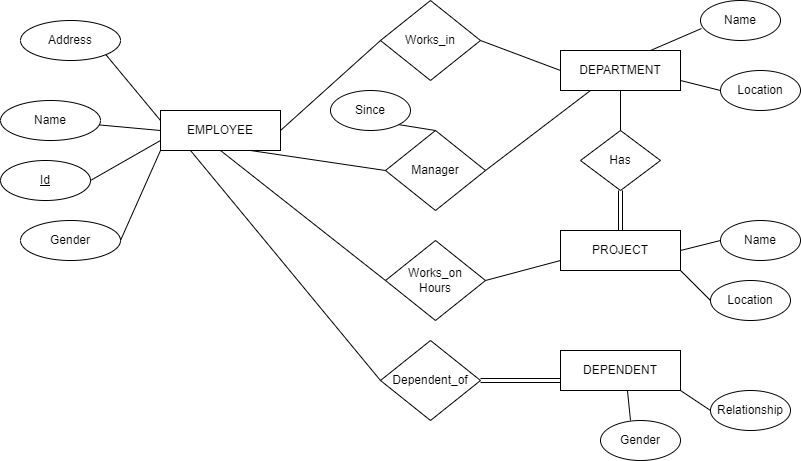
\includegraphics[width=12cm]{img/erdiagram.png}
    \caption{ER Diagram}
    
\end{figure}

\section{Features and functions}
The employee management system project provides several features
and functions to meet the needs of HR personnel, managers, and
employees. The following are some of the key features and functions of
the system: 
\begin{enumerate}
    \item Employee Data Management: The system allows HR personnel to
manage employee data, including personal information, contact
details, emergency contacts, performance evaluations, and
benefits administration. The system provides a centralized
database that stores all employee information, ensuring that it is
up-to-date and accessible to authorized personnel.
\item Time and Attendance Tracking: The system provides a time and
attendance tracking module that allows employees to clock in and
out, and managers to track their attendance. The system provides
real-time data on employee attendance, enabling managers to
identify attendance issues and take corrective action.
\item Leave Management: The system allows employees to request time
off and managers to approve or reject their requests. The system
provides real-time data on employee leave requests, allowing
managers to allocate resources effectively and ensure that the
workload is distributed evenly. 
\item Performance Evaluation: The system provides a performance
evaluation module that allows managers to track employee
performance and provide feedback. The system provides real-time
data on employee performance, allowing managers to identify
areas for improvement and take corrective action. 
\item Benefits Administration: The system provides a benefits
administration module that allows HR personnel to manage
employee benefits, such as health insurance, retirement plans, and
other perks. The system provides real-time data on employee
benefits, allowing HR personnel to make informed decisions and
allocate resources effectively.
\item Communication Tools: The system provides communication tools
that allow employees to communicate with their managers and HR
personnel, providing feedback, requesting assistance, and
receiving updates. The system provides a centralized
communication platform that ensures that all communication is
recorded and accessible to authorized personnel.
\end{enumerate}
Overall, the employee management system project provides a
comprehensive set of features and functions that streamline HR
processes, improve data management, and enhance the employee
experience
\end{document}
